\documentclass[tikz,border=0pt]{standalone}
\usepackage[T1]{fontenc}
\usepackage{helvet}
\renewcommand{\familydefault}{\sfdefault}
\usetikzlibrary{arrows.meta,calc}
\tikzset{
 flow/.style={-{Stealth[length=1.7mm,width=1.1mm]},line width=.5pt},
 pics/truck/.style={code={
   % Identical orthographic tractor/trailer geometry for all powertrains.
   \draw (0,2)--(0,7)--(2.5,10)--(7,10)--(7,2)--cycle;
   \draw (1.1,7.2)--(3,9.1)--(5.8,9.1)--(5.8,7.2)--cycle;
   \draw (1,5.8)--(2.4,5.8) (6.2,5.6)--(6.2,6.2);
   \draw (8,3.5) rectangle (29,11);
   \draw (7,2)--(29,2) (8,2)--(8,3.5);
   \foreach \x in {3.5,12,24,27}{
     \draw[fill=white] (\x,1.7) circle (1.65);
     \draw (\x,1.7) circle (.65);
   }
 }},
 metric/.style={draw,minimum width=58mm,minimum height=13mm,inner sep=0pt}
}
\begin{document}
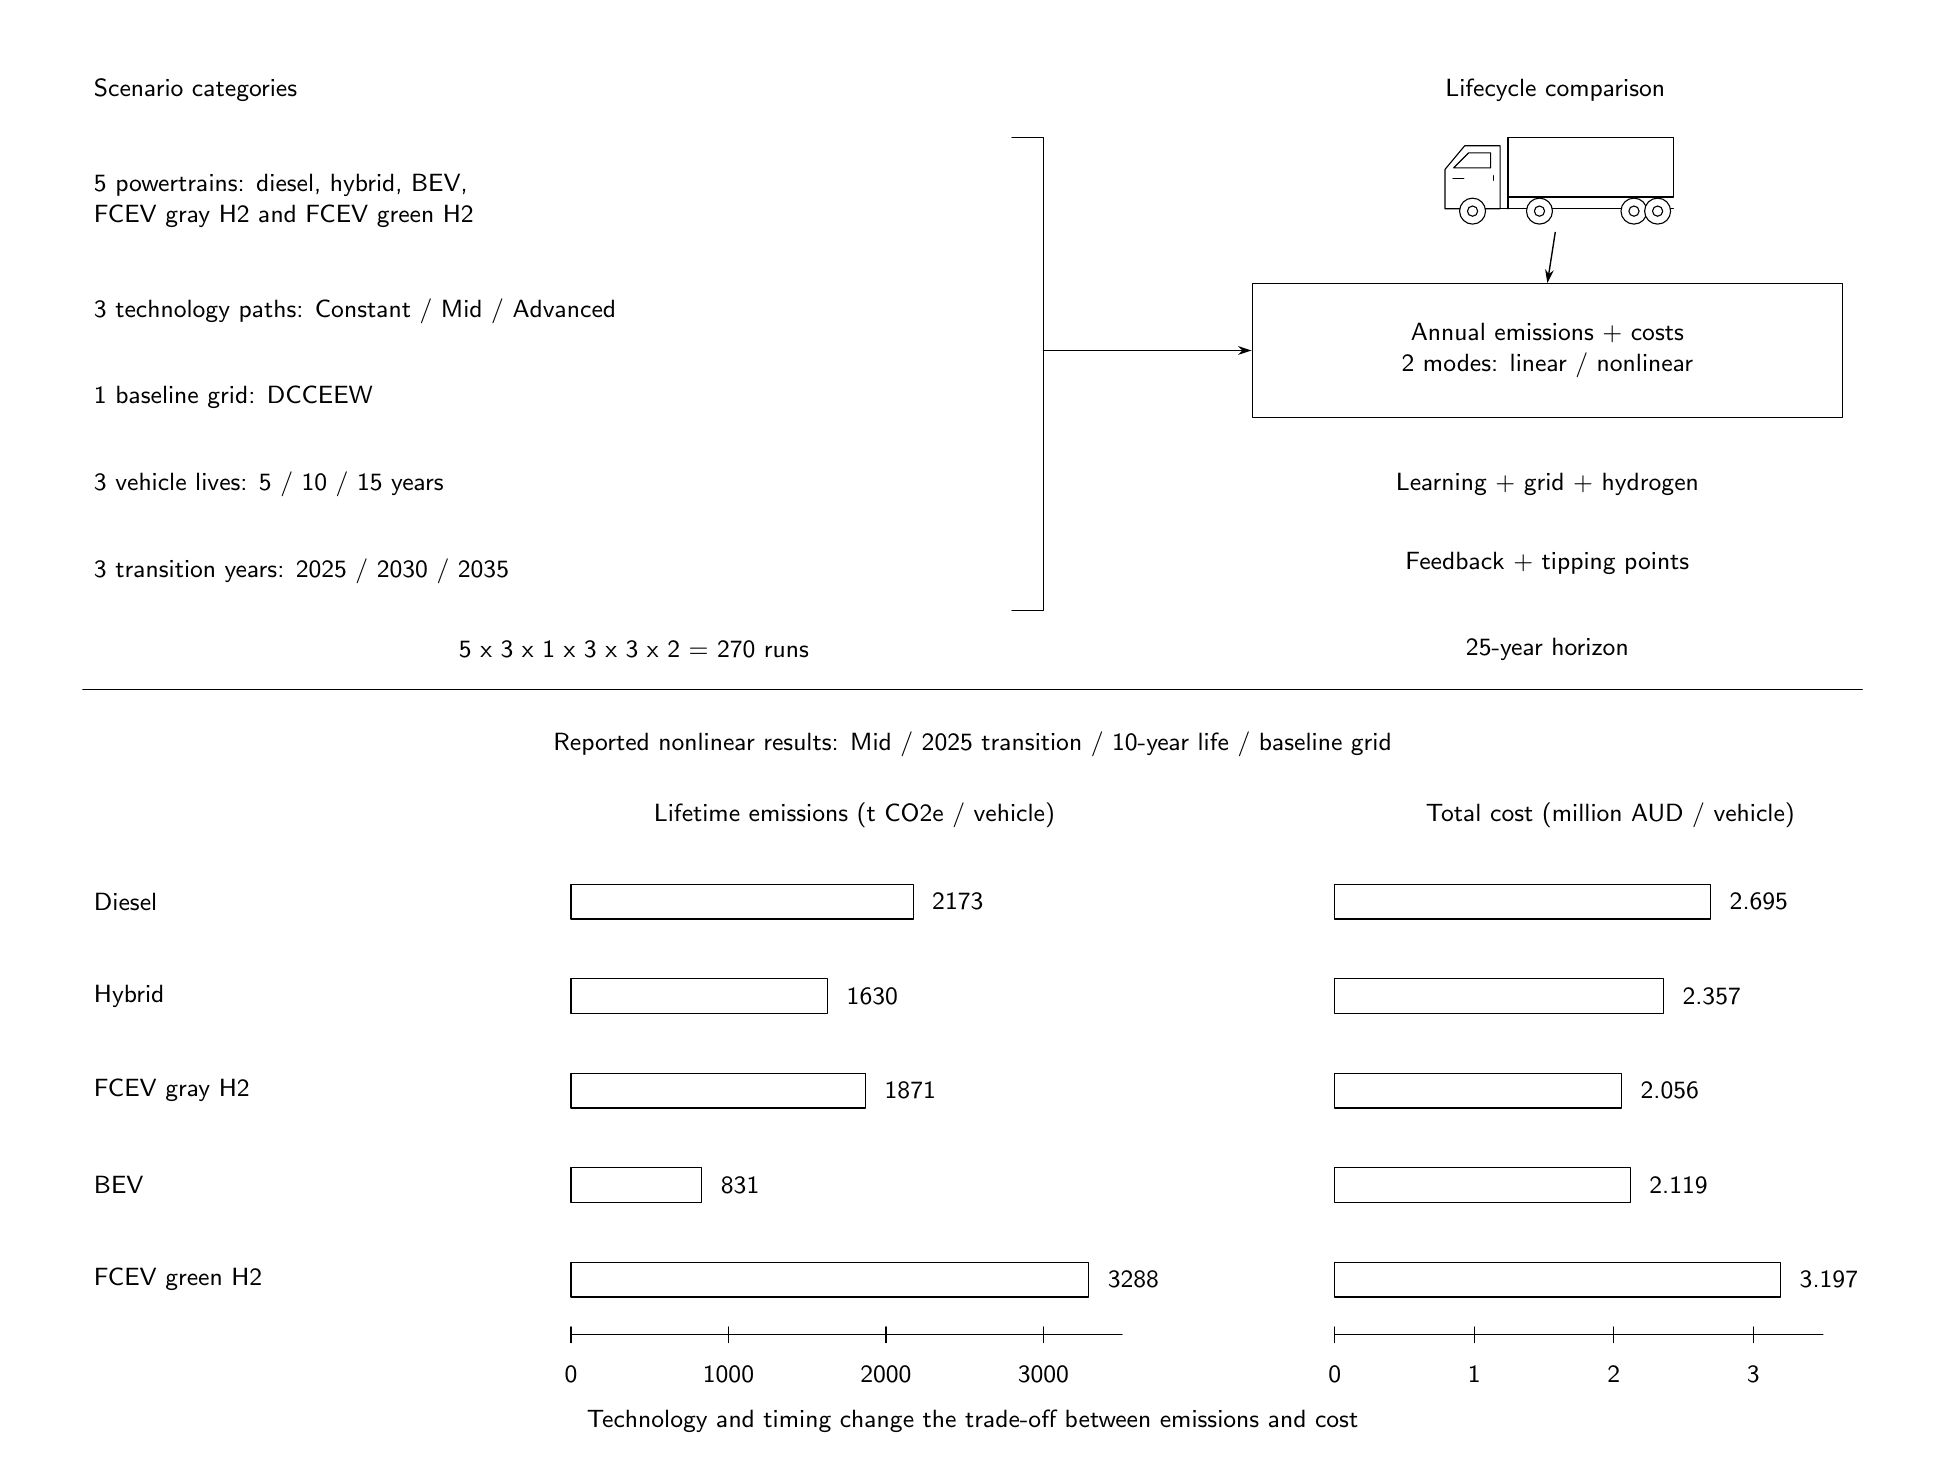
\begin{tikzpicture}[x=1mm,y=1mm,line width=.4pt,line cap=round,line join=round,
 every node/.style={font=\fontsize{9}{11}\selectfont,inner sep=1pt}]
\path[use as bounding box] (0,0) rectangle (240,180);
\node[anchor=west] at (8,172) {Scenario categories};
\node[anchor=west,align=left] at (8,158) {5 powertrains: diesel, hybrid, BEV,\\FCEV gray H2 and FCEV green H2};
\node[anchor=west] at (8,144) {3 technology paths: Constant / Mid / Advanced};
\node[anchor=west] at (8,133) {1 baseline grid: DCCEEW};
\node[anchor=west] at (8,122) {3 vehicle lives: 5 / 10 / 15 years};
\node[anchor=west] at (8,111) {3 transition years: 2025 / 2030 / 2035};
\pic at (180,155) {truck};
\node at (194,172) {Lifecycle comparison};
\node[draw,align=center,minimum width=75mm,minimum height=17mm]
 (model) at (193,139) {Annual emissions + costs\\2 modes: linear / nonlinear};
\draw[flow] (194,154)--(model.north);
\node at (193,122) {Learning + grid + hydrogen};
\node at (193,112) {Feedback + tipping points};
\draw (125,166)--(129,166)--(129,106)--(125,106);
\draw[flow] (129,139)--(model.west);
\node at (193,101) {25-year horizon};
\node at (77,101) {5 x 3 x 1 x 3 x 3 x 2 = 270 runs};
\draw (7,96)--(233,96);
\node at (120,89) {Reported nonlinear results: Mid / 2025 transition / 10-year life / baseline grid};
\node at (105,80) {Lifetime emissions (t CO2e / vehicle)};
\node at (201,80) {Total cost (million AUD / vehicle)};
% Replot of Table 1; deterministic scenario values, no invented uncertainty.
\foreach \name/\yy/\em/\cost in {Diesel/69/2173/2.695,Hybrid/57/1630/2.357,FCEV gray H2/45/1871/2.056,BEV/33/831/2.119,FCEV green H2/21/3288/3.197}{
 \node[anchor=west] at (8,\yy) {\name};
 \draw (69,\yy-2.2) rectangle ({69+(\em/3500)*70},\yy+2.2);
 \node[anchor=west] at ({71+(\em/3500)*70},\yy) {\em};
 \draw (166,\yy-2.2) rectangle ({166+62*\cost/3.5},\yy+2.2);
 \node[anchor=west] at ({168+62*\cost/3.5},\yy) {\cost};
}
\draw (69,14)--(139,14) (166,14)--(228,14);
\foreach \v in {0,1000,2000,3000}{
 \draw ({69+(\v/3500)*70},13)--({69+(\v/3500)*70},15);
 \node at ({69+(\v/3500)*70},9) {\v};
}
\foreach \v in {0,1,2,3}{
 \draw ({166+62*\v/3.5},13)--({166+62*\v/3.5},15);
 \node at ({166+62*\v/3.5},9) {\v};
}
\node at (120,3) {Technology and timing change the trade-off between emissions and cost};
\end{tikzpicture}
\end{document}
